\documentclass[25pt, a0paper, portrait, margin=0mm, innermargin=20mm,
blockverticalspace=2mm, colspace=20mm, subcolspace=0mm]{tikzposter} %Default values for poster format options.

\input{packages}

\definecolor{unired}{HTML}{a51e37}
\definecolor{mypink1}{rgb}{0.858, 0.188, 0.478}
\definecolor{mblack}{HTML}{0d0d0d}
\definecolor{titlecolor}{RGB}{74, 114, 159}
\definecolor{titledarkcolor}{RGB}{51,102,153}
\definecolor{Grey}{HTML}{e1e1e1}
\definecolor{DarkerGrey}{RGB}{215,217,219}
\definecolor{FontColor}{HTML}{0d0d0d}
\definecolor{Red}{RGB}{204,0,0}
\definecolor{L-lig}{RGB}{25,124,192}
\definecolor{point-lig}{RGB}{255,255,255}
\definecolor{G-lig}{RGB}{62,66,68}

\definecolor{Orange}{RGB}{240,163,10} 
\definecolor{LightRed}{RGB}{214,98,93}
\definecolor{LightBlue}{RGB}{160,200,217}
\definecolor{LightGreen}{RGB}{130,161,119}
\definecolor{Violet}{RGB}{190,144,252}

\colorlet{blocktitlefgcolor}{mblack}
\colorlet{backgroundcolor}{Grey}
\colorlet{blocktitlebgcolor}{Grey}
\colorlet{blockbodyfgcolor}{FontColor}
\colorlet{innerblocktitlebgcolor}{L-lig}
\colorlet{innerblocktitlefgcolor}{white}
\colorlet{notefrcolor}{white}
\colorlet{notefgcolor}{black}
\colorlet{notebgcolor}{white}




\begin{document}
 
\renewcommand{\baselinestretch}{1} 
\title{\parbox{1500pt}{Motion blindness induced by color in zebrafish larvea \textit{Danio rerio}}}
\author{Alexander Wendt, Patrick Weygoldt}
\institute{Systems Neurobiology, Department of Neurobiology, University of Tuebingen}
\usetitlestyle[]{sampletitle}
\maketitle
\renewcommand{\baselinestretch}{1.4} 

\begin{columns}
\column{0.3333}
\myblock[MyBlock]{Introduction}{
   Color has a big influence on motion vision in zebrafish. 
   Michael B. Orger (2004) displayed that zebrafish in behavioural experiments show motion blindness 
   to a grating of different colors, but little is known about the cortical structures conveing the
   \glqq color-motion\grqq{} perception. We wanted to the investigate the 
   optic tectum of the zebrafish larvae with calcium imaging. 
    \vspace{0.6cm}
    \begin{tikzfigure}[]
        \label{griddrawing}
        \includegraphics[width=\linewidth]{figs/dsc_2193_02.jpg}
    \end{tikzfigure} 
}

\myblock[MyBlock]{Preprocessing:}{
    \textbf{1. Region of Interests (ROI):} corrosponds to neurons with 
    genetically encoded caclium indicators. The lumiance $f$ of the calcium imaging is calculated from the change of luminance normalized to the average luminance $f = \frac{\Delta f}{f}$.   
    
    \vspace{0.6}

    \begin{minipage}{.07\textwidth}
    \begin{tikzfigure}[]
        \label{Rois}
        \includegraphics[width=8cm]{figs/Screenshot 2022-11-17 at 19.05.14.png}
    \end{tikzfigure} 
    \end{minipage}
    \begin{minipage}{.26\textwidth}
    \begin{tikzfigure}[]
        \label{Raw}
        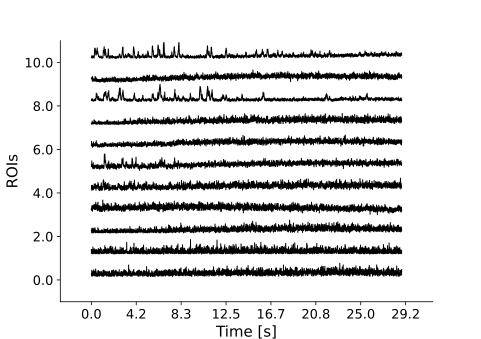
\includegraphics[width=14cm]{figs/raw2.pdf}
    \end{tikzfigure} 
    \end{minipage}

    \vspace{0.6cm}
    \textbf{2. Active ROIs:}
    To get the active ROIs we computed the correlation within 3 repeats of the same stimulus.  
    \vspace{0.6}

    \begin{minipage}{0.07\textwidth}
    \begin{tikzfigure}[]
        \label{Rois}
        \includegraphics[width=10cm]{figs/}
    \end{tikzfigure} 
    \end{minipage}
    \begin{minipage}{.26\textwidth}
    \begin{tikzfigure}[]
        \label{Raw}
        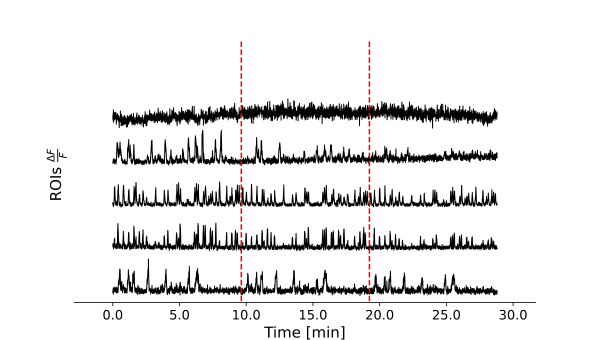
\includegraphics[width=14cm]{figs/autocorrelation.pdf}
    \end{tikzfigure} 
    \end{minipage} 


    }

\column{0.6666}
\myblock[MyBlock]{Detected modulations}{
    
    We found phases of synchrony up to 50 Hz in $\Delta$EOD$f$ that lasted for over 10 minutes. 
    Synchronous modulations ranged from clearly distinguishable and steep rises to smooth modulations with low EOD$f$ increases.

    \vspace{0.4cm}

    \begin{tikzfigure}[]
        \label{modulations}
        \includegraphics[width=\linewidth]{figs/selected_modulations.pdf}
    \end{tikzfigure}
    \vspace{0.2cm}
    \begin{tikzfigure}[]
        \label{eventpos}
        \includegraphics[width=\linewidth]{figs/eventposition_2.pdf}
    \end{tikzfigure} 

    \noindent
}

\myblock[MyBlock]{Interactions at modulations}{
    \vspace{-1.2cm}
    \begin{tikzfigure}[]
        \label{results}
        \includegraphics[width=\linewidth]{figs/eventstats.pdf}
    \end{tikzfigure}

    \begin{multicols}{2}
        \begin{itemize}
            \setlength\itemsep{0.5em}
            \item $\Delta$EOD$f$ does not appear to decrease during synchronous modulations (\textbf{A}).
            \item Individuals that rise their EOD$f$ first appear to rise their frequency higher compared to reactors (\textbf{B}).
            \vfill
            \null
            \columnbreak
            \item Synchronized fish keep distances below 1 m (\textbf{C}) but distances over 3 m also occur (see \textbf{movie}).
            \item Spatial interactions increase \textbf{after} the start of a synchronous modulation (\textbf{D}).
        \end{itemize}
    \end{multicols}
    \vspace{-1cm}
}

\myblock[MyBlock]{Conclusion}{
    \begin{itemize}
        \setlength\itemsep{0.5em}
        \item Our analysis is the first to indicate that \textit{A. leptorhynchus} uses long, diffuse and synchronized EOD$f$ signals to communicate in addition to chirps and rises.
        \item The recorded fish do not exhibit jamming avoidance behavior while close during synchronous modulations.
        \item Synchronous signals \textbf{initiate} spatio-temporal interactions.
    \end{itemize}
    \vspace{0.2cm}
    }
\end{columns}

\node [above right, text=white, outer sep=45pt,minimum width=\paperwidth, align=center, draw, fill=unired, color=unired] at (-43.6,-61) { \textcolor{white}{\normalsize Contact: patrick.weygoldt@student.uni-tuebingen.de}};

\end{document}